\def\linkdethi{} %Đường link cần dẫn tới
\anmaQR
%%%%%%%%%%%%%%%%%%%%%%%%
\def\toanlop{12}
\def\thoigian{90}
\def\namhoc{2025 - 2026}
\begin{dethi}
	{Bộ GD\&ĐT}
	{VTED ft KING EDU}
	{TDMT03}
	{Đề thi thử THPTQG 2026}
\end{dethi}
\caulc
\Opensolutionfile{ans}[ans/ansTN-Dung]
%%%=============EX_1=============%%%
\begin{ex}%[1D1H5-3]%[TDMT03]%[Nguyễn Trí Minh Tuấn]
	Nghiệm của phương trình $\cos x=\dfrac{1}{2}$ là
	\choice
	{\True $x=\pm\dfrac{\pi}{3}+k2\pi$, $k\in\mathbb{Z}$}
	{$x=\pm\dfrac{\pi}{3}+k\pi$, $k\in\mathbb{Z}$}
	{$\hoac{&x=\dfrac{\pi}{6}+k2\pi\\&x=\dfrac{5\pi}{6}+k2\pi}$, $k\in\mathbb{Z}$}
	{$x=\pm\dfrac{\pi}{6}+k2\pi$, $k\in\mathbb{Z}$}
	\loigiai{
		Ta có $\cos x=\dfrac{1}{2} \Leftrightarrow \cos x=\cos\dfrac{\pi}{3} \Leftrightarrow x=\pm\dfrac{\pi}{3}+k2\pi$, $k\in\mathbb{Z}$.
	}
\end{ex}
%%%=============================%%%

%%%=============EX_2=============%%%
\begin{ex}%[1D6N3-3]%[TDMT03]%[Trần Văn Thiện]
	Hàm số nào dưới đây đồng biến trên $\mathbb{R}$?
	\choice
	{$y=\ln x$}
	{$y=x^2$}
	{\True $y=\mathrm{e}^x$}
	{$y=x^3-3x$}
	\loigiai{
		Ta thấy hàm số $y=\mathrm{e}^x$ có dạng $y=a^x$ với $a=\mathrm{e}>1$ nên là hàm số đồng biến trên $\mathbb{R}$.
	}
\end{ex}
%%%=============================%%%

%%%=============EX_3=============%%%
\begin{ex}%[1D5H1-3]%[TDMTD01]%[Phạm Hải Dương]
	Cho hai mẫu số liệu ghép nhóm $M_1$, $M_2$ với bảng tần số ghép nhóm như sau\\
	Nhóm $M_1$
	\begin{center}
		\begin{tabular}{|c|c|c|c|c|c|c|}
			\hline
			Nhóm $M_1$ & $[5;7)$ & $[7;9)$ & $[9;11)$ & $[11;13)$ & $[13;15)$ & $[15;17)$ \\
			\hline
			Tần số & $3$ & $5$ & $6$ & $4$ & $6$ & $7$ \\
			\hline
		\end{tabular}
	\end{center}
	Nhóm $M_2$
	\begin{center}
		\begin{tabular}{|c|c|c|c|c|c|c|}
			\hline
			Nhóm $M_2$ & $[5;7)$ & $[7;9)$ & $[9;11)$ & $[11;13)$ & $[13;15)$ & $[15;17)$ \\
			\hline
			Tần số & $3$ & $10$ & $6$ & $4$ & $6$ & $12$ \\
			\hline
		\end{tabular}
	\end{center}
	Hãy so sánh số trung bình cộng $\overline{x}_1$, $\overline{x}_2$ của hai mẫu số liệu $M_1$, $M_2$?
	\choice
	{$\overline{x}_1=2\overline{x}_2$}
	{$\overline{x}_1=\overline{x}_2$}
	{\True $\overline{x}_1<\overline{x}_2$}
	{$\overline{x}_1=3\overline{x}_2$}
	\loigiai{
		Nhóm $M_1$
		\begin{center}
			\begin{tabular}{|c|c|c|c|c|c|c|}
				\hline
				Giá trị đại diện & $6$ & $8$ & $10$ & $12$ & $14$ & $16$ \\
				\hline
				Tần số & $3$ & $5$ & $6$ & $4$ & $6$ & $7$ \\
				\hline
			\end{tabular}
		\end{center}
		Giá trị trung bình $\overline{x}_1=\dfrac{6\cdot3+8\cdot5+10\cdot6+12\cdot4+14\cdot6+16\cdot7}{3+5+6+4+6+7}=\dfrac{362}{31}\approx 11{,}68$.\\
		Nhóm $M_2$
		\begin{center}
			\begin{tabular}{|c|c|c|c|c|c|c|}
				\hline
				Giá trị đại diện & $6$ & $8$ & $10$ & $12$ & $14$ & $16$\\
				\hline
				Tần số & $3$ & $10$ & $6$ & $4$ & $6$ & $12$ \\
				\hline
			\end{tabular}
		\end{center}
		Giá trị trung bình $\overline{x}_2=\dfrac{6\cdot3+8\cdot10+10\cdot6+12\cdot4+14\cdot6+16\cdot7}{3+10+6+4+6+12}=\dfrac{382}{41}\approx 11{,}76$.\\
		Ta thấy $\overline{x}_1<\overline{x}_2$.
	}
\end{ex}
%%%=============================%%%

%%%=============EX_4=============%%%
\begin{ex}%[2D1H3-1]%[TDMT03]%[Văn Minh Thoại]
	Hãy tính $\min\limits_{[0;3]}\left(x^3-3x^2\right)$?
	\choice
	{$0$}
	{$1$}
	{\True $-4$}
	{$2$}
	\loigiai{
		Xét hàm số $y=x^3-3x^2$ có
		$y'=3x^2-6x=0\Leftrightarrow\hoac{&x=0\in[0;3]\\&x=2\in[0;3].}$\\
		Bảng biến thiên
		\begin{center}
			
\begin{tikzpicture}
				\tkzTabInit[nocadre=false,lgt=1.2,espcl=2.5,deltacl=0.6]
				{$x$ /0.7, $y'$ /0.7, $y$ /2}
				{$0$, $2$, $3$}
				\tkzTabLine {,- , 0 , + ,}
				\tkzTabVar {+/$0$,-/$-4$,+/$0$}
			\end{tikzpicture}
		\end{center}
		Dựa vào bảng biến thiên ta thấy $\min\limits_{[0;3]}\left(x^3-3x^2\right)=-4$.
	}
\end{ex}
%%%=============================%%%

%%%=============EX_5=============%%%
\begin{ex}%[2D1N4-1]%[TDMT03]%[Lê Phúc]
	\immini[thm]{Cho hàm số $y=\dfrac{ax+b}{cx+d}$ ($c\neq0$, $ad\ne bc$) có đồ thị như hình vẽ. Tiệm cận ngang của đồ thị hàm số đó là
		\choice
		{$y=1$}
		{$x=2$}
		{\True $y=2$}
		{$x=1$}
	}{
		\begin{tikzpicture}[line join=round,line cap=round, font=\footnotesize,scale=0.5,>=stealth]
			\draw[-stealth](-2.5,0)--(5,0)node[above]{$x$};
			\draw[-stealth](0,-2)--(0,5)node[left]{$y$};		
			\draw[smooth,samples=300,domain=1.25:4.5] plot(\x,{(2*\x-3)/(\x-1)});
			\draw[smooth,samples=300,domain=-2.4:0.65] plot(\x,{(2*\x-3)/(\x-1)});
			\draw[dashed,smooth,samples=300,domain=-2.5:4.6] plot(\x,2);	
			\fill (0,0) circle(1pt)node[below left]{$O$};
			\draw[dashed](1,-2)--(1,5);
			\foreach \x/\g in {1/-120}\fill[black] (\x,0) circle (1pt)+(\g:.4)node{$\x$};	
			\foreach \x/\g in {2/210}\fill[black] (0,\x) circle (1pt)+(\g:.4)node[below ]{$\x$};		
		\end{tikzpicture}
	}
	\loigiai{
		Dựa vào đồ thị hàm số ta thấy $y=2$ là tiệm cận ngang.
	}
\end{ex}
%%%=============================%%%

%%%=============EX_6=============%%%
\begin{ex}%[1D6N4-2]%[TDMT03]%[Vũ Hồng Toàn]
	Nghiệm của phương trình $\log(x-1)=1$ tương ứng là
	\choice
	{$x=2$}
	{\True $x=11$}
	{$x=9$}
	{$x=3$}
	\loigiai{
		Điều kiện $x-1>0\Leftrightarrow x>1$.\\
		Phương trình $\log(x-1)=1\Leftrightarrow x-1=10\Leftrightarrow x=11$.\\
		Đối chiếu điều kiện, phương trình đã cho có nghiệm là $x=11$.
	}
\end{ex}
%%%=============================%%%

%%%=============EX_7=============%%%
\begin{ex}%[2D1H2-2]%[TDMT03]%[Chu Ha]
	Cho hàm số $f(x)$ có bảng biến thiên đạo hàm $f'(x)$ như sau
	\begin{center}
		
\begin{tikzpicture}
			\tkzTabInit[nocadre=false,lgt=1.2,espcl=2.5,deltacl=0.6]
			{$x$ /0.7, $f''(x)$ /0.7, $f'(x)$ /2}
			{$-\infty$, $-4$, $0$, $1$, $+\infty$}
			\tkzTabLine {,+,z,- , z , + ,z,-,}
			\tkzTabVar {-/$-\infty$,+/$5$,-/$0$,+/$2$,-/$-\infty$}
		\end{tikzpicture}
	\end{center}
	Hàm số $f(x)$ có tất cả bao nhiêu điểm cực trị?
	\choice
	{$0$}
	{$1$}
	{\True $2$}
	{$3$}
	\loigiai{
		Dựa vào bảng biến thiên ta thấy đường thẳng $y=0$ cắt $y=f'(x)$ tại hai điểm phân biệt và tiếp xúc tại một điểm (hai nghiệm đơn và một nghiệm kép $x=0$.\\
		Hàm số $f(x)$ có hai điểm cực trị.
	}
\end{ex}
%%%=============================%%%

%%%=============EX_8=============%%%
\begin{ex}%[TDM31]%[1H8H2-3]
	Cho hình chóp $S.ABCD$ có đáy $ABCD$ là hình chữ nhật, có $SA \perp (ABCD)$. Trong các cặp đường thẳng cho dưới đây, cặp nào \textbf{không} vuông góc với nhau?
	\choice
	{$SA$, $BC$}
	{$SA$, $BD$}
	{\True $SC$, $BC$}
	{$SB$, $BC$}
	\loigiai{
		\immini{Ta có $\heva{& BC \perp AB \\ & BC \perp SA} \Rightarrow BC \perp (SAB) \Rightarrow BC \perp SB$.\\
		Mặt khác, vì $SA \perp (ABCD)$ nên $SA \perp BC$ và $SA \perp BD$.\\
		Suy ra các cặp $(SA, BC)$, $(SA, BD)$ và $(SB, BC)$ đều vuông góc với nhau.\\
		Vậy cặp đường thẳng $SC$, $BC$ \textbf{không} vuông góc với nhau.}{
		\begin{tikzpicture}[scale=1, font=\footnotesize, line join=round, line cap=round, >=stealth]
			\coordinate (A) at (0,0);
			\coordinate (B) at (-1.5,-1.5);
			\coordinate (D) at (3,0);
			\coordinate (C) at (1.5,-1.5);
			\coordinate (S) at (0,2.5);
			\draw[dashed] (S)--(A)--(B) (A)--(D);
			\draw (S)--(B)--(C)--(D)--(S) (S)--(C);
			\fill (S) circle (1pt) node[above] {$S$};
			\fill (A) circle (1pt) node[above right] {$A$};
			\fill (B) circle (1pt) node[left] {$B$};
			\fill (C) circle (1pt) node[below] {$C$};
			\fill (D) circle (1pt) node[right] {$D$};
			\draw pic[draw, angle radius=2mm] {right angle=S--B--C};
		\end{tikzpicture}}
	}
\end{ex}
%%%=============================%%%

%%%=============EX_9=============%%%
\begin{ex}%[1D6N4-2]%[Đỗ Đường Hiếu]
	Nghiệm của phương trình $4^x=32$ là
	\choice
	{$x=5$}
	{$x=3$}
	{\True $x=\dfrac{5}{2}$}
	{$x=8$}
	\loigiai{
		Phương trình $4^x=32\Leftrightarrow 2^{2x}=2^5\Leftrightarrow 2x=5\Leftrightarrow x=\dfrac{5}{2}$.
	}
\end{ex}
%%%=============================%%%

%%%=============EX_10=============%%%
\begin{ex}%[1D2N3-3]%[TDMT03]%[Huỳnh Quốc Đạt]
	Cho cấp số nhân $\left(u_n\right)$ có $u_1=1$ và công bội $q=2$. Số hạng $u_4$ bằng
	\choice
	{$7$}
	{$9$}
	{$16$}
	{\True $8$}
	\loigiai{
		Ta có $u_4=u_1\cdot q^3=1\cdot2^3=8$.
	}
\end{ex}
%%%=============================%%%

%%%=============EX_11=============%%%
\begin{ex}%[2H2N1-1]%[TDMTD03]%[Dương Công Tạo]
	\immini[thm]{Cho hình hộp $ABCD. A'B'C'D'$. Hỏi phát biểu nào dưới đây đúng?
		\choice
		{$\overrightarrow{AB}+\overrightarrow{AC}+\overrightarrow{AA'}=\overrightarrow{AC'}$}
		{$\overrightarrow{AB}+\overrightarrow{A'D}+\overrightarrow{AA'}=\overrightarrow{AC'}$}
		{$\overrightarrow{AB}+\overrightarrow{BC}+\overrightarrow{C'C'}=\overrightarrow{AC'}$}
		{\True $\overrightarrow{AB}+\overrightarrow{AD}+\overrightarrow{AA'}=\overrightarrow{AC'}$}
	}{
		\begin{tikzpicture}[declare function={a=2; b=0.45*a; h=0.65*a;}]
			\path (0:0) coordinate (A)
			(220:b) coordinate (B)
			($(B)+(a,0)$) coordinate (C)
			(a,0) coordinate (D)
			\foreach \x in {A,B,C,D}{(\x)++(90:h) coordinate (\x1)};
			\draw[dashed] (A1)--(A)--(B) (A)--(D);
			\draw (B1)--(A1)--(D1)--(C1) (D1)--(D)--(C) (B)--(C)--(C1)--(B1)--cycle;
			\foreach \x/\goc/\t in {A/45/A,B/-90/B,C/-90/C,D/0/D,A1/90/A',B1/90/B',C1/90/C',D1/90/D'}
			\fill (\x) circle (1pt) node[shift={(\goc:7pt)},font=\scriptsize]{$\t$};
		\end{tikzpicture}
	}
	\loigiai{
		Theo quy tắc hình hộp ta có $\overrightarrow{AB}+\overrightarrow{AD}+\overrightarrow{AA'}=\overrightarrow{AC'}$.
	}
\end{ex}
%%%=============================%%%

%%%=============EX_12=============%%%
\begin{ex}%[2D1H2-1]
	Hàm số $y=\dfrac{x^2-2x-3}{x-1}$.
	\choice
	{Đạt cực đại tại $x=-1$}
	{Đạt cực tiểu tại $x=1$}
	{\True Không có cực trị}
	{Nghịch biến trên từng khoảng xác định}
	\loigiai
	{
		Tập xác định $\mathscr{D}=\mathbb{R}\setminus\{1\}$.\\
		Đạo hàm $y'=\dfrac{x^2-2x+5}{(x-1)^2}$.\\
		Cho $y'=0\Leftrightarrow x^2-2x+5=0$ vô nghiệm, mà $a=1>0$ nên $y'>0,\,\forall x\in \mathscr{D}$.\\
		Vậy hàm số không có cực trị.
	}
\end{ex}
%%%=============================%%%
\Closesolutionfile{ans}

\cauds
\Opensolutionfile{ans}[ans/ansTN-DungSai]
%%%=============EX_13=============%%%
\begin{ex}%[2D1H3-1]%[Duong Xuan Loi]
	Cho hàm số $f(x)=x^2+4\cos x$.
	\choiceTF[t]
	{$f'(x)=2x+4\sin x$}
	{\True $f''(x)=2-4\cos x$}
	{\True Hàm số $f(x)$ nghịch biến trên khoảng $\left(0;\dfrac{\pi}{2}\right)$}
	{\True $\max\limits_{\left[0;\tfrac{\pi}{2}\right]}f(x)=4$}
	\loigiai{
		\begin{itemchoice}
			\itemch $f'(x)=2x-4\sin x$.
			\itemch $f''(x)=2-4\cos x$.
			\itemch Xét $x\in\left(0;\dfrac{\pi}{2}\right)$, ta có $f''(x)=2-4\cos x=0\Leftrightarrow \cos x=\dfrac{1}{2}\Leftrightarrow x=\dfrac{\pi}{3}$.\\
			$x=\dfrac{\pi}{3}\Rightarrow f'(x)=\dfrac{2\pi}{3}-2\sqrt{3}\approx -1{,}37$.\\
			$x=\dfrac{\pi}{2}\Rightarrow f'(x)=\pi-4\approx -0{,}86$.\\
			Bảng biến thiên
			\begin{center}
				
\begin{tikzpicture}
					\tkzTabInit[nocadre=false,lgt=1.2,espcl=3.5,deltacl=0.7]
					{$x$ /1, $f''(x)$ /0.7, $f'(x)$ /2}
					{$0$, $\dfrac{\pi}{3}$, $\dfrac{\pi}{2}$}
					\tkzTabLine {,-,z,+,}
					\tkzTabVar {+/$0$,-/$-1{,}37$,+/$-0{,}86$}
				\end{tikzpicture}
			\end{center}
			Do đó trên khoảng $\left(0;\dfrac{\pi}{2}\right)$ thì $f'(x)<0$ nên hàm số $f(x)$ nghịch biến.
			\itemch Do hàm số $f(x)$ nghịch biến trên $\left[0;\dfrac{\pi}{2}\right]$ nên $\max\limits_{\left[0;\tfrac{\pi}{2}\right]}f(x)=f(0)=4$.
		\end{itemchoice}
	}
\end{ex}
%%%=============================%%%

%%%=============EX_14=============%%%
\begin{ex}%[Vovanle]%[TDM-KSCL-DE3]%[1H8V6-2]
	Cho hình chóp đều $S. ABCD$ có cạnh đáy bằng $4$ và chiều cao bằng $6$.
	\choiceTF[t]
	{\True Thể tích của hình chóp $S. ABCD$ bằng $32$}
	{\True $\mathrm{d}(S,(ABC))=6$}
	{$\mathrm{d}(A,(SBC))=2\sqrt{3}$}
	{Số đo góc nhị diện $[A,SB,C]$ bằng $113^{\circ}$ (\textit{làm tròn kết quả đến hàng đơn vị})}
	\loigiai{
		\begin{center}
			\begin{tikzpicture}[scale=1, font=\footnotesize, line join=round, line cap=round, >=stealth]
				\def\a{3}
				\path
				(0,0) coordinate (A)
				(0:\a) coordinate (B)
				(230:0.6*\a) coordinate (D)	
				($(B)+(D)$) coordinate (C)
				($(A)!0.5!(C)$) coordinate (O)
				($(B)!0.5!(C)$) coordinate (M)
				($(O)!2!90:(M)$) coordinate (S)
				($(S)!0.7!(M)$) coordinate (H)
				($(S)!0.4!(B)$) coordinate (K)	
				;
				\draw (S)--(B)--(C)--(D)--(S)--(C)(M)--(S)(K)--(C);
				\draw[dashed] (S)--(A)--(B)(A)--(D)--(B)(A)--(C)(S)--(O)--(M)(O)--(H)(A)--(K)--(O);	
				\foreach \x/\g in {S/90,A/-90,B/0,C/-30,D/180,O/-90,M/-20,H/60,K/60}\fill[black] (\x) circle (1pt)+(\g:.3)node{$\x$};
			\end{tikzpicture}
		\end{center}
		\noindent Gọi $O$ là tâm hình vuông $ABCD$.\\
		Do $S.ABCD$ là hình chóp đều nên $SO$ là đường cao.
		\begin{itemchoice}
			\itemch Thể tích hình chóp là $V=\dfrac{1}{3}SO\cdot S_{ABCD}=\dfrac{1}{3}\cdot 6\cdot 4^2=32$.
			\itemch Ta có $\mathrm{d}(S,(ABC))=\mathrm{d}(S,(ABCD))=SO=6$.
			\itemch Gọi $M$ là trung điểm của $BC$, $H$ là hình chiếu của $O$ lên $SM$.\\
			Ta có $\heva{&BC\perp OM\\&BC\perp SO}\Rightarrow BC\perp (SOM)$.\\
			Mà $OH\subset (SOM)$ nên $OH\perp BC$.\\
			Khi đó $\heva{&OH\perp SM\\&OH\perp BC}\Rightarrow OH\perp (SBC)$.\\
			Suy ra $\mathrm{d}(O,(SBC))=OH$.\\
			Tam giác $SOM$ vuông tại $O$ nên ta có\\
			$\dfrac{1}{OH^2}=\dfrac{1}{OM^2}+\dfrac{1}{SO^2}=\dfrac{1}{2^2}+\dfrac{1}{6^2}=\dfrac{5}{18}\Rightarrow OH=\dfrac{3\sqrt{10}}{5}$.\\
			$\mathrm{d}(A,(SBC))=2\mathrm{d}(O,(SBC))=2OH=2\cdot \dfrac{3\sqrt{10}}{5}=\dfrac{6\sqrt{10}}{5}$.
			\itemch Gọi $K$ là hình chiếu của $A$ lên $SB$.\\
			Ta có $\heva{&AK\perp SB\\&AC\perp SB}\Rightarrow SB \perp (AKC)\Rightarrow CK\perp SB\Rightarrow [A,SB,C]=\widehat{AKC}$.\\
			Ta có $\dfrac{1}{OK^2}=\dfrac{1}{OB^2}+\dfrac{1}{SO^2}=\dfrac{1}{\left(2\sqrt{2}\right)^2}+\dfrac{1}{6^2}=\dfrac{11}{72}\Rightarrow OK=\dfrac{6\sqrt{22}}{11}$.\\
			$\tan \widehat{OKC}=\dfrac{OC}{OK}=\dfrac{2\sqrt{2}}{\dfrac{6\sqrt{22}}{11}}=\dfrac{\sqrt{11}}{3}\Rightarrow \widehat{OKC}\approx 48^\circ$.\\
			Ta có $[A,SB,C]=\widehat{AKC}=2\widehat{OKC}=2\cdot 48^\circ=96^\circ$.
		\end{itemchoice}
	}
\end{ex}
%%%=============================%%%

%%%=============EX_15=============%%%
\begin{ex}%[2D1V5-7]%[TDMT03]%[Lê Hồ Quang Minh]
	Cho hàm số $f(x)=\dfrac{x+2}{x-1}$ có đồ thị $(C)$.
	\choiceTF[t]
	{\True Đồ thị $(C)$ có tiệm cận đứng là $x=1$ và tiệm cận ngang là $y=1$}
	{\True Đồ thị $(C)$ có tâm đối xứng là $I(1;1)$}
	{\True Đồ thị hàm số $y=xf(x)$ có tiệm cận xiên là $y=x+3$}
	{\True Gọi $A$, $B$, $C$, $D$ là $4$ điểm phân biệt có tọa độ nguyên thuộc $(C)$. Một điểm $M$ chạy trong mặt phẳng $Oxy$. Giá trị nhỏ nhất của biểu thức $MA+MB+MC+MD$ là $4\sqrt{10}$}
	\loigiai{
		\begin{itemchoice}
			\itemch Ta có $\lim\limits_{x\to 1^-}y=-\infty$; $\lim\limits_{x\to 1^+}y=+\infty$, suy ra $x=1$ là tiệm cận đứng.\\
			$\lim\limits_{x\to -\infty}y=1$; $\lim\limits_{x\to +\infty}y=1$, suy ra $y=1$ là tiệm cận ngang.
			\itemch Tâm đối xứng là giao điểm của hai tiệm cận $I(1;1)$.
			\itemch Hàm số $y=xf(x)=\dfrac{x^2+2x}{x-1}=x+3+\dfrac{3}{x-1}$ có tiệm cận xiên là $y=x+3$.
			\itemch Hàm số $y=f(x)=\dfrac{x+2}{x-1}=1+\dfrac{3}{x-1}$.\\
			Đồ thị hàm số có tọa độ nguyên khi và chỉ khi $x-1$ là ước của $3$. Khi đó
			\begin{itemize}
				\item $x-1=1\Leftrightarrow x=2\Rightarrow y=4$, ta được điểm $A(2;4)$.
				\item $x-1=-1\Leftrightarrow x=0\Rightarrow y=-2$, ta được điểm $C(0;-2)$.
				\item $x-1=3\Leftrightarrow x=4\Rightarrow y=2$, ta được điểm $B(4;2)$.
				\item $x-1=-3\Leftrightarrow x=-2\Rightarrow y=0$, ta được điểm $D(-2;0)$.
			\end{itemize}
			Ta thấy $\overrightarrow{AB}=\left(2;-2\right)$; $\overrightarrow{DC}=\left(2;-2\right)$ nên $\overrightarrow{AB}=\overrightarrow{DC}$.\\
			Suy ra $ABCD$ là hình bình hành tâm $I\left(1;1\right)$.\\
			Mặt khác $AC=BD=2\sqrt{10}$ nên $ABCD$ là hình chữ nhật.\\
			Do đó $MA+MB+MC+MD \ge AC+BD$, dấu ``='' xảy ra khi $M$ là giao điểm hai đường chéo, tức $M\equiv I$.\\
			Vậy $MA+MB+MC+MD$ nhỏ nhất bằng $4IA=4\sqrt{\left(2-1\right)^2+\left(4-1\right)^2}=4\sqrt{10}$.
		\end{itemchoice}
	}
\end{ex}
%%%=============================%%%

%%%=============EX_16=============%%%
\begin{ex}%[2D1V3-6]%[TDMT03]%[Lương Pho]
	Từ một miếng bìa hình vuông cạnh bằng $60$\,cm, người ta cắt bỏ $4$ phần ở $4$ góc như hình vẽ và giữ lại một mảnh được tô hai màu (gồm $1$ hình vuông cạnh $x$ và $4$ tam giác cân). Tiến hành gấp mảnh còn lại thành một hình chóp tứ giác đều ($T$).
	\begin{center}
		\begin{tikzpicture}[scale=.65,declare function={a=6; x=2.6; shiftx=9.5;}, line join=round, line cap=round, every node/.style={font=\large}]
			\path
			(-a/2,-a/2) coordinate (BL)
			(a/2,-a/2) coordinate (BR)
			(a/2,a/2) coordinate (TR)
			(-a/2,a/2) coordinate (TL)
			(-x/2,-x/2) coordinate (Sq1)
			(x/2,-x/2) coordinate (Sq2)
			(x/2,x/2) coordinate (Sq3)
			(-x/2,x/2) coordinate (Sq4)
			(0,a/2) coordinate (TipT)
			(a/2,0) coordinate (TipR)
			(0,-a/2) coordinate (TipB)
			(-a/2,0) coordinate (TipL);
			\fill[orange!25] (Sq1) -- (Sq2) -- (Sq3) -- (Sq4) -- cycle;
			\fill[cyan!30] (Sq4) -- (Sq3) -- (TipT) -- cycle;
			\fill[cyan!30] (Sq3) -- (Sq2) -- (TipR) -- cycle;
			\fill[cyan!30] (Sq2) -- (Sq1) -- (TipB) -- cycle;
			\fill[cyan!30] (Sq1) -- (Sq4) -- (TipL) -- cycle;
			\draw[line width=0.6pt] (BL) rectangle (TR);
			\draw[line width=0.6pt] (Sq1) -- (Sq2) -- (Sq3) -- (Sq4) -- cycle;
			\draw[line width=0.6pt] (Sq4) -- (TipT) -- (Sq3);
			\draw[line width=0.6pt] (Sq3) -- (TipR) -- (Sq2);
			\draw[line width=0.6pt] (Sq2) -- (TipB) -- (Sq1);
			\draw[line width=0.6pt] (Sq1) -- (TipL) -- (Sq4);
			\node at (-a/3.3,a/3.3) {\textit{Bỏ}};
			\node at (a/3.3,a/3.3) {\textit{Bỏ}};
			\node at (-a/3.3,-a/3.3) {\textit{Bỏ}};
			\node at (a/3.3,-a/3.3) {\textit{Bỏ}};
			\node[above=-2pt] at (0,x/2) {$x$};
			\draw[Stealth-Stealth,line width=0.6pt] (-a/2,-a/2 - 0.5) -- (a/2,-a/2 - 0.5) node[midway,below] {$60$\,cm};
			\path (a/2 + 0.8,0.5) coordinate (ArL);
			\draw[line width=0.6pt] (ArL) ++(0,0.2) -- ++(1.2,0) -- ++(0,0.25) -- ++(0.5,-0.45) -- ++(-0.5,-0.45) -- ++(0,0.25) -- ++(-1.2,0) -- cycle;
			\node[above right] at ($(ArL) + (0.85,0.5)$) {\textit{Gấp thành}};
			\path
			(shiftx - 2,-1.5) coordinate (PA)
			(shiftx + 1.5,-1.5) coordinate (PB)
			(shiftx + 3.2,0.2) coordinate (PC)
			(shiftx - 0.3,0.2) coordinate (PD)
			(shiftx + 0.6,3.2) coordinate (PS);
			\fill[orange!25] (PA) -- (PB) -- (PC) -- (PD) -- cycle;
			\draw[dashed,line width=0.6pt] (PA) -- (PD) -- (PC);
			\draw[dashed,line width=0.6pt] (PS) -- (PD);
			\draw[line width=0.6pt] (PA) -- (PB) -- (PC) -- (PS) -- cycle;
			\draw[line width=0.6pt] (PS) -- (PB);
			\draw[line width=0.6pt] (PS) -- (PA);
			\node[below] at ($(PA)!0.5!(PB)$) {$x$};
		\end{tikzpicture}
	\end{center}
	\choiceTF[t]
	{\True Điều kiện của $x$ là $0<x<30$}
	{Diện tích của phần bị cắt đi là $S_{\text{cắt}}=60x$ ($\mathrm{cm}^2$)}
	{Thể tích của khối chóp ($T$) là $V=120x-x^3$ ($\mathrm{cm}^3$)}
	{Thể tích của khối chóp ($T$) lớn nhất khi $x=15$\,cm}
	\loigiai{
		\immini{
			Gọi $S.ABCD$ là hình chóp tứ giác đều được tạo thành với tâm đáy là $O$. Gọi $M, N$ lần lượt là trung điểm của hai cạnh đáy đối diện $CD$ và $AB$.\\
			Khi đó $MN = x$ và trung đoạn của hình chóp là $SM = SN = y > 0$.\\
			Từ hình trải phẳng, đường thẳng nối hai đỉnh của hai tam giác cân đối diện đi qua tâm hình vuông và có độ dài bằng cạnh miếng bìa $60$\,cm. Do đó
			\[ SM + MN + SN = 60 \Leftrightarrow 2y + x = 60 \Leftrightarrow y = \dfrac{60-x}{2}. \]
		}{
			\begin{tikzpicture}[font=\scriptsize]
				\tikzset{declare function={a=5; b=3; h=4.5;}}
				\path (0,0) coordinate (A)
				(a,0) coordinate (D)
				(-135:b) coordinate (B)
				($(B)+(D)$) coordinate (C)
				($(A)!0.5!(C)$) coordinate (O)
				($(O)+(0,h)$) coordinate (S)
				($(C)!0.5!(D)$) coordinate (M)
				($(A)!0.5!(B)$) coordinate (N);
				\foreach \x/\y/\z in {A/O/S,D/O/S}{
					\path (\y) pic[draw,angle radius=5pt]{right angle = \x--\y--\z};
				}
				\draw[dashed] (B)--(A)--(D)--cycle (C)--(A)--(S)--(O)
				(S)--(N)--(M);
				\draw (S)--(B)--(C)--(D)--cycle (S)--(C)
				(S)--(M);
				\foreach \t/\g in {A/150,B/-90,C/-60,D/60,S/90,O/-90,M/0,N/180}{
					\fill (\t) circle (1pt) node[shift={(\g:7pt)},font=\scriptsize]{$\t$};
				}
			\end{tikzpicture}
		}		
		\begin{itemchoice}
			\itemch Trong tam giác $SMN$ ta có bất đẳng thức tam giác
			\[ SM+SN>MN\Leftrightarrow 2y>x\Leftrightarrow 2\cdot\dfrac{60-x}{2}>x\Leftrightarrow x<30. \]
			Kết hợp $x>0$, điều kiện của $x$ là $0<x<30$.
			\itemch Diện tích toàn phần của hình chóp là
			\[ S_{\text{tp}}=4S_{\triangle SBC}+S_{ABCD}=4\cdot\dfrac{1}{2}xy+x^2=2x\cdot\dfrac{60-x}{2}+x^2=60x. \]
			Diện tích phần bị cắt đi là $S_{\text{cắt}} = S_{\text{bìa}} - S_{\text{tp}} = 60^2 - 60x = 3\,600 - 60x$.
			\itemch Chiều cao khối chóp là
			\[ SO^2 = SM^2 - OM^2 = y^2 - \left(\dfrac{x}{2}\right)^2 = \left(\dfrac{60-x}{2}\right)^2 - \dfrac{x^2}{4} = \dfrac{3\,600-120x}{4} = 900-30x. \]
			Thể tích khối chóp là $V = \dfrac{1}{3}SO\cdot S_{ABCD} = \dfrac{1}{3}x^2\sqrt{900-30x}$.
			\itemch Ta có hàm thể tích
			\[ V = \dfrac{1}{3}x^2\sqrt{900-30x} = \dfrac{1}{3}\sqrt{(900-30x)x^4} = \dfrac{1}{3}\sqrt{900x^4-30x^5}. \]
			Đặt $f(x)=900x^4-30x^5$, với $0<x<30$.\\
			Ta có $f'(x)=3\,600x^3-150x^4$. Xét $f'(x)=0 \Leftrightarrow x=24$ (do $x>0$).\\
			Bảng biến thiên
			\begin{center}
				
\begin{tikzpicture}
					\tkzTabInit[nocadre=false,lgt=1.2,espcl=3.5,deltacl=0.5]
					{$x$ /0.7, $f'(x)$ /0.7, $f(x)$ /2}
					{$0$, $24$, $30$}
					\tkzTabLine {,+,0,-,}
					\tkzTabVar {-/,+/,-/}
				\end{tikzpicture}
			\end{center}
			Dựa vào bảng biến thiên, suy ra $\max\limits_{(0;30)} f(x)=f(24)$ tại $x=24$.\\
			Vậy thể tích của khối chóp ($T$) đạt giá trị lớn nhất khi $x=24$\,cm.
		\end{itemchoice}
	}
\end{ex}
%%%=============================%%%
\Closesolutionfile{ans}

\caukq 
\Opensolutionfile{ans}[ans/ansTN-DienKhuyet]
%%%=============EX_17=============%%%
\begin{ex}%[1H8V5-4]%[TDMT03]%[Võ Hiệp]
	Cho hình chóp $S. ABC$ có đáy là tam giác $ABC$ đều cạnh bằng $6$, $SA=3$ và vuông góc với đáy. Tính khoảng cách giữa hai đường thẳng $SB$ và $AC$ (\textit{làm tròn kết quả đến hàng phần mười}).
	\par
	\shortans[oly]{2{,}6}
	\loigiai{
		\immini{
			Gọi $D$ là đỉnh thứ tư của hình bình hành $ACBD$.\\
			Ta có $\heva{&AC\parallel BD\\&BD\subset (SBD)}\Rightarrow AC\parallel (SBD)$.\\
			Do đó $\mathrm{d}(AC,SB)=\mathrm{d}\big(AC,(SBD)\big)=\mathrm{d}\big(A,(SBD)\big)$.\\
			Gọi $H$ là trung điểm của $BD$, $K$ là hình chiếu của $A$ trên $SH$.\\
			Do $ACBD$ là hình bình hành và $\triangle ABC$ đều nên $\triangle ABD$ đều. Khi đó
			\[ \heva{&BD\perp AH\\&BD\perp SA} \Rightarrow BD\perp (SAH). \]
			Mà $AK \subset (SAH)$ nên $AK\perp BD$.\\
			Suy ra $\heva{&AK\perp SH\\&AK\perp BD}\Rightarrow AK\perp (SBD)$.\\
			Nên $\mathrm{d}\big(A,(SBD)\big)=AK$.\\
			Vì $\triangle ABD$ đều cạnh bằng $6$ nên $AH=\dfrac{BD\sqrt{3}}{2}=\dfrac{6\sqrt{3}}{2}=3\sqrt{3}$.\\
			Tam giác $SAH$ vuông tại $A$ có $AK\perp SH$, suy ra
			\[ \dfrac{1}{AK^2}=\dfrac{1}{SA^2}+\dfrac{1}{AH^2}=\dfrac{1}{3^2}+\dfrac{1}{\left(3\sqrt{3}\right)^2}=\dfrac{4}{27} \Rightarrow AK=\sqrt{\dfrac{27}{4}}=\dfrac{3\sqrt{3}}{2}. \]
			Vậy $\mathrm{d}(AC,SB)=AK=\dfrac{3\sqrt{3}}{2}\approx 2{,}6$.
		}{
			\begin{tikzpicture}[declare function={a=3.5; b=2; h=3.5; goc=-140;}, line join=round, line cap=round, >=stealth, font=\footnotesize, scale=0.9]
				\path
				(0,0) coordinate (A)
				(0:a) coordinate (D)
				(goc:b) coordinate (C)	
				($(D)+(C)$) coordinate (B)	
				($(A)+(0,h)$) coordinate (S)
				($(B)!0.5!(D)$) coordinate (H)
				($(S)!(A)!(H)$) coordinate (K);
				
				\draw[dashed] (S)--(A) (A)--(C) (A)--(D) (A)--(B) (A)--(H) (A)--(K);
				\draw (S)--(C)--(B)--(D)--cycle (S)--(B) (S)--(H);
				
				\path pic[draw,angle radius=4pt]{right angle=A--H--D};
				\path pic[draw,angle radius=4pt]{right angle=A--K--S};
				\path pic[draw,angle radius=4pt]{right angle=S--A--D};
				
				\foreach \p/\g in {S/90, A/135, B/-90, C/-135, D/0, H/-30, K/30}
				\filldraw (\p) circle (1pt) node[shift={(\g:3mm)}] {$\p$};
			\end{tikzpicture}
		}
	}
\end{ex}
%%%=============================%%%

%%%=============EX_18=============%%%
\begin{ex}%[2D1V3-6]%[TDMT03]%[Nguyễn Đức Tuấn Anh]
	Giả sử chi phí để sản xuất $x$ đơn vị của một loại hàng hoá nào đó được cho bởi hàm số $C(x)=x^3-59x^2+1\,300x$ (nghìn đồng). Hãy xác định chi phí biên nhỏ nhất theo đơn vị nghìn đồng (\textit{làm tròn kết quả đến hàng đơn vị})?
	\par
	\shortans[oly]{140}
	\loigiai{
		Hàm chi phí biên $C'(x)=3x^2-118x+1\,300$.\\
		Ta có $C''(x)=6x-118$, $C''(x)=0\Leftrightarrow x=\dfrac{59}{3}$.\\
		Bảng biến thiên
		\begin{center}
			
\begin{tikzpicture}
				\tkzTabInit[nocadre=false,lgt=1.4,espcl=4,deltacl=0.6]
				{$x$ /1, $C''(x)$ /0.7, $C'(x)$ /2.2}
				{$0$, $\dfrac{59}{3}$, $+\infty$}
				\tkzTabLine {,-,z,+,}
				\tkzTabVar {+/,-/$\dfrac{419}{3}$,+/}
			\end{tikzpicture}
		\end{center}
		Vậy chi phí biên nhỏ nhất là $\dfrac{419}{3}\approx 140$ (ngàn đồng).
	}
\end{ex}
%%%=============================%%%

%%%=============EX_19=============%%%
\begin{ex}%[2D1V3-2]%[TDMT03]%[Bồ Văn Hậu]
	Cho hình chóp tứ giác đều $S.ABCD$. Gọi $\alpha$ và $\beta$ lần lượt là góc giữa mặt bên với đáy và góc giữa cạnh bên với đáy. Hãy tính theo đơn vị độ giá trị lớn nhất của $(\alpha-\beta)$ \textit{(làm tròn kết quả đến hàng phần mười)}?
	\par 
	\shortans[oly]{9,9}
	\loigiai{
		\immini{
			Gọi $O$ là tâm hình vuông $ABCD$.\\
			Do $S.ABCD$ là hình chóp tứ giác đều nên $SO\perp (ABCD)$.\\
			Có $OB$ là hình chiếu của $SB$ lên $(ABCD)$, suy ra $\big(SB,(ABCD)\big)=\widehat{SBO}=\beta$.\\
			Gọi $M$ là trung điểm của $BC$.\\
			Khi đó
			$\heva{&BC\perp OM\\&BC\perp SO}\Rightarrow BC\perp (SOM)\Rightarrow BC\perp SM$.\\
			Ta có $\heva{&(ABCD)\cap(SBC)=BC\\&BC\perp OM\\&BC\perp SM}$,
			suy ra $\big((SBC),(ABCD)\big)=\widehat{SMO}=\alpha$.\\
			Đặt $OM=x>0\Rightarrow OB=x\sqrt{2}$; $SO=kx$ (với $k>0$).\\
			Ta có $\tan\alpha=\dfrac{SO}{OM}=\dfrac{kx}{x}=k$, $\tan\beta=\dfrac{SO}{OB}=\dfrac{kx}{x\sqrt{2}}=\dfrac{k}{\sqrt{2}}$.
		}{
			\begin{tikzpicture}[declare function={a=4; b=2; h=3.5; goc=220;}, line join=round, line cap=round, >=stealth, font=\footnotesize, scale=0.9]
				\path
				(0,0) coordinate (A)
				(a,0) coordinate (B)
				(goc:b) coordinate (D)	
				($(B)+(D)$) coordinate (C)
				($(A)!0.5!(C)$) coordinate (O)
				($(B)!0.5!(C)$) coordinate (M)
				($(O)+(0,h)$) coordinate (S);
				\draw[dashed] (S)--(A) (A)--(B) (A)--(D) (A)--(C) (B)--(D) (S)--(O) (O)--(M);
				\draw (S)--(B)--(C)--(D)--cycle (S)--(C) (S)--(M);
				\path pic[draw,angle radius=12pt, angle eccentricity=1.4, "$\beta$"] {angle = S--B--O}; 
				\path pic[draw,angle radius=12pt, angle eccentricity=1.4, "$\alpha$"] {angle = S--M--O}; 
				\path pic[draw,angle radius=4pt] {right angle= S--O--M};
				\foreach \x/\g in {S/90, A/135, B/0, C/-45, D/180, O/-90, M/0}
				\filldraw (\x) circle (1pt) node[shift={(\g:3mm)}] {$\x$};
			\end{tikzpicture}
		}
		Ta có
		\[ \tan(\alpha-\beta)=\dfrac{\tan\alpha-\tan\beta}{1+\tan\alpha\tan\beta}=\dfrac{k-\dfrac{k}{\sqrt{2}}}{1+k\cdot\dfrac{k}{\sqrt{2}}}=\dfrac{k\left(\sqrt{2}-1\right)}{k^2+\sqrt{2}}=\dfrac{\sqrt{2}-1}{\dfrac{k^2+\sqrt{2}}{k}}. \]
		Đặt $f(k)=\dfrac{k^2+\sqrt{2}}{k}$, với $k>0$.\\
		Suy ra $f'(k)=\dfrac{k^2-\sqrt{2}}{k^2}=0\Rightarrow k=\sqrt[4]{2}$.\\
		Bảng biến thiên
		\begin{center}
			
\begin{tikzpicture}
				\tkzTabInit[nocadre=false,lgt=1.2,espcl=3.5,deltacl=0.6]
				{$k$ /1, $f'(k)$ /0.7, $f(k)$ /2}
				{$0$, $\sqrt[4]{2}$, $+\infty$}
				\tkzTabLine {,-,z,+,}
				\tkzTabVar {+/,-/,+/}
			\end{tikzpicture}
		\end{center}
		Để $(\alpha-\beta)$ lớn nhất thì $\tan(\alpha-\beta)$ lớn nhất hay $f(k)$ nhỏ nhất.\\
		Dựa vào bảng biến thiên, ta thấy $f(k)$ nhỏ nhất khi $k=\sqrt[4]{2}$.\\
		Lúc này $\tan(\alpha-\beta)=\dfrac{k\left(\sqrt{2}-1\right)}{k^2+\sqrt{2}}=\dfrac{\sqrt[4]{2}\left(\sqrt{2}-1\right)}{\left(\sqrt[4]{2}\right)^2+\sqrt{2}} \Rightarrow (\alpha-\beta) \approx 9{,}9^\circ$.
	}
\end{ex}
%%%=============================%%%

%%%=============EX_20=============%%%
\begin{ex}%[TDMT03]%[1D2V3-8]
	Một chú bò X được chăn trên một ruộng cỏ có diện tích bằng $180$ m$^2$. Biết rằng ngày đầu tiên chú bò này ăn hết $12$ m$^2$ cỏ và những ngày sau đó sức ăn của chú bò tăng lên $5\%$ so với ngày ngay trước đó. Với giả thiết rằng một đám cỏ bị ăn thì sau $7$ đêm sẽ mọc lại như cũ và lại tiếp tục ăn được (còn chưa qua đủ $7$ đêm thì sẽ không ăn được), mỗi sáng sớm ra ruộng cỏ nếu diện tích cỏ ít hơn khả năng ăn của chú bò ngày hôm đó thì chú bò sẽ được chăn ở ruộng cỏ khác. Hãy tính số ngày mà chú bò đã ăn ở ruộng cỏ ban đầu?
	\par
	\shortans[oly]{19}
	\loigiai{
		Gọi $u_1$, $u_2$, $u_3$,\ldots, $u_k$ lần lượt là diện tích mà chú bò ăn từ ngày thứ $1$, $2$, $3$, \ldots, $k$.\\
		Kể từ ngày thứ $8$ thì diện tích cỏ bị ăn là $u_8$ và diện tích cỏ mọc lại và ăn được là $u_1$.\\
		Sáng ngày thứ $8$ diện tích cỏ bò ăn được là
		\[180-\left(u_1+u_2+u_3+\ldots+u_7\right)+u_1=180-\left(u_2+u_3+\ldots+u_7\right).\]
		Sáng ngày thứ $k$ ($k\geqslant8$) thì diện tích cỏ bò ăn được là $180-\left(u_{k-6}+u_{k-5}+u_{k-4}+\ldots+u_{k-1}\right)$.\\
		Để chú bò sang đám ruộng khác ăn thì $180-\left(u_{k-6}+u_{k-5}+u_{k-4}+\ldots+u_{k-1}\right)<u_k$.\\
		Theo đề bài ta có diện tích cỏ bị ăn mỗi ngày theo cấp số nhân có công bội $q=1{,}05$.\\
		Do đó ta có
		\allowdisplaybreaks
		\begin{eqnarray*}
			&&180-\left(u_{k-6}+u_{k-5}+u_{k-4}+\ldots+u_{k-1}\right)< u_k\\
			&\Leftrightarrow& 180-\left(u_{k-6}+u_{k-5}+u_{k-4}+\ldots+u_{k-1}+u_k\right)<0\\
			&\Leftrightarrow& 180-u_{k-6}\left(1+q+q^2+\ldots+q^6\right)<0\\
			&\Leftrightarrow& 180-u_1q^{k-7}\cdot\dfrac{1-q^7}{1-q}<0\\
			&\Leftrightarrow& 180-12\cdot1{,}05^{k-7}\cdot\dfrac{1-1{,}05^7}{1-1{,}05}<0\\
			&\Leftrightarrow& 1{,}05^{k-7}>\dfrac{180\cdot0{,}05}{12\cdot \left(1{,}05^7-1\right)}\\
			&\Leftrightarrow& k-7>\log_{1{,}05}\dfrac{180\cdot0{,}05}{12\cdot \left(1{,}05^7-1\right)}\\
			&\Leftrightarrow& k>19{,}52.
		\end{eqnarray*}
		Từ đó suy ra $k=20$ là ngày đầu tiên lượng cỏ không đủ để chú bò ăn nên phải chuyển sang ruộng khác.\\
		Vậy chú bò đã ăn ở ruộng cỏ ban đầu trọn vẹn $20-1=19$ ngày.
	}
\end{ex}
%%%=============================%%%

%%%=============EX_21=============%%%
\begin{ex}%[Nguyễn Văn Sang]%[TDM-KSCL-DE3]%[0D0V2-6]
	\immini[thm]{
		Trên mặt phẳng tọa độ $Oxy$, cho hình tròn $(C)$ có bán kính bằng $10$ tiếp xúc với hai trục tọa độ $Ox$, $Oy$. Hình vuông $(V)$ nội tiếp đường tròn $(C)$ có các cạnh song song với các trục tọa độ. Chọn ngẫu nhiên một điểm có tọa độ nguyên nằm trong hình tròn $(C)$. Hãy tính xác suất để điểm được chọn thuộc hình phẳng được tô màu (\textit{làm tròn kết quả đến hàng phần trăm})?
	}{
		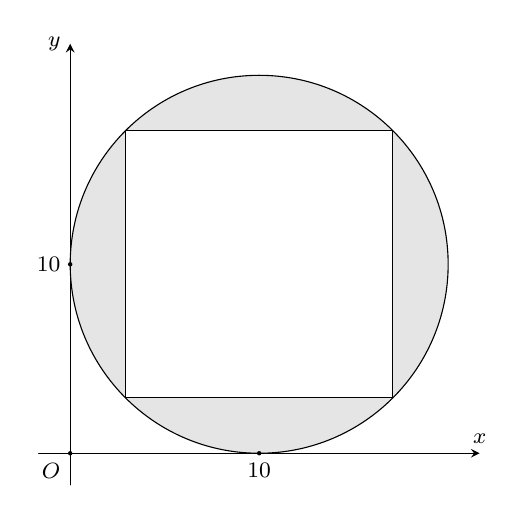
\begin{tikzpicture}[declare function={r=3; s=r/sqrt(2);}, line join=round, line cap=round, font=\footnotesize, scale=0.8, >=stealth]
			\coordinate (I) at (r,r);
			\coordinate (A) at (r-s,r-s);
			\coordinate (B) at (r-s,r+s);
			\coordinate (C) at (r+s,r+s);
			\coordinate (D) at (r+s,r-s);
			\draw[-stealth] (-0.5,0) -- (2*r+0.5,0) node[above] {$x$};
			\draw[-stealth] (0,-0.5) -- (0,2*r+0.5) node[left] {$y$};
			\fill[black!10] (I) circle (r);
			\fill[white] (A) -- (B) -- (C) -- (D) -- cycle;
			\draw (I) circle (r);
			\draw (A) -- (B) -- (C) -- (D) -- cycle;
			\fill (0,0) circle (1pt) node[below left] {$O$};
			\fill (r,0) circle (1pt) node[below] {$10$};
			\fill (0,r) circle (1pt) node[left] {$10$};
		\end{tikzpicture}
	}
	\par
	\shortans[0]{0{,}29}
	\loigiai{
		Phương trình hình tròn $(C)$ (bao gồm cả biên) là $(x-10)^2+(y-10)^2 \leqslant 100$.\\
		Hình vuông nội tiếp đường tròn có đường chéo là $2R=20$, do đó độ dài cạnh là $10\sqrt{2}$.\\
		Phần tô màu gồm 4 hình viên phân bằng nhau.
		\immini{
			Xét viên phân phía dưới (giới hạn bởi cung tròn và cạnh đáy của hình vuông). Các điểm nguyên thuộc phần này thỏa mãn
			\[ \heva{&0 \leqslant y < 10-5\sqrt{2} \approx 2{,}93 \\ &(x-10)^2+(y-10)^2 \leqslant 100.} \]
			Do $y$ nguyên nên $y \in \{0; 1; 2\}$. Ta có:
			\begin{itemize}
				\item Với $y=0$: $(x-10)^2 \leqslant 0 \Leftrightarrow x=10$ (có $1$ điểm).
				\item Với $y=1$: $(x-10)^2 \leqslant 19 \Leftrightarrow 10-\sqrt{19} \leqslant x \leqslant 10+\sqrt{19}$ \\
				$\Rightarrow x \in \{6; 7; \ldots; 14\}$ (có $9$ điểm).
				\item Với $y=2$: $(x-10)^2 \leqslant 36 \Leftrightarrow 10-6 \leqslant x \leqslant 10+6$ \\
				$\Rightarrow x \in \{4; 5; \ldots; 16\}$ (có $13$ điểm).
			\end{itemize}
			Suy ra số điểm nguyên thuộc một viên phân là $1+9+13=23$ điểm.\\
			Dễ thấy 4 viên phân đôi một không có tọa độ nguyên nào trùng nhau, nên số điểm nguyên thuộc phần tô màu (biến cố $A$) là $n(A) = 23 \cdot 4 = 92$ điểm.
		}{
			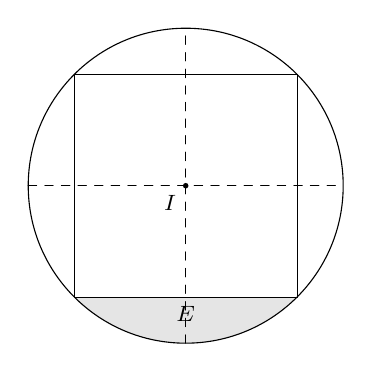
\begin{tikzpicture}[declare function={r=2; s=r/sqrt(2);}, line join=round, line cap=round, font=\footnotesize, scale=1, >=stealth]
				\coordinate (I) at (r,r);
				\coordinate (A) at (r-s,r-s);
				\coordinate (D) at (r+s,r-s);
				\fill[black!10] (A) arc (225:315:r) -- cycle;
				\draw (I) circle (r);
				\draw (r-s,r-s) -- (r+s,r-s) -- (r+s,r+s) -- (r-s,r+s) -- cycle;
				\draw[dashed] (r,0) -- (r,2*r) (0,r) -- (2*r,r);
				\fill (I) circle (1pt) node[below left] {$I$};
				\node[below] at (r, r-s) {$E$};
			\end{tikzpicture}
		}
		\noindent
		Tiếp theo, ta đếm tổng số điểm nguyên nằm trong toàn bộ hình tròn $(C)$ bằng cách xét $y \in \{0; 1; \ldots; 20\}$:
		\begin{itemize}
			\item $y=0, y=20$: mỗi trường hợp có $1$ điểm ($x=10$).
			\item $y=1, y=19$: mỗi trường hợp có $9$ điểm ($x \in \{6; \ldots; 14\}$).
			\item $y=2, y=18$: mỗi trường hợp có $13$ điểm ($x \in \{4; \ldots; 16\}$).
			\item $y=3, y=17$: $(x-10)^2 \leqslant 51 \Rightarrow x \in \{3; \ldots; 17\}$, mỗi trường hợp có $15$ điểm.
			\item $y=4, y=16$: $(x-10)^2 \leqslant 64 \Rightarrow x \in \{2; \ldots; 18\}$, mỗi trường hợp có $17$ điểm.
			\item $y=5, y=15$: $(x-10)^2 \leqslant 75 \Rightarrow x \in \{2; \ldots; 18\}$, mỗi trường hợp có $17$ điểm.
			\item $y=6, y=14$: $(x-10)^2 \leqslant 84 \Rightarrow x \in \{1; \ldots; 19\}$, mỗi trường hợp có $19$ điểm.
			\item $y=7, y=13$: $(x-10)^2 \leqslant 91 \Rightarrow x \in \{1; \ldots; 19\}$, mỗi trường hợp có $19$ điểm.
			\item $y=8, y=12$: $(x-10)^2 \leqslant 96 \Rightarrow x \in \{1; \ldots; 19\}$, mỗi trường hợp có $19$ điểm.
			\item $y=9, y=11$: $(x-10)^2 \leqslant 99 \Rightarrow x \in \{1; \ldots; 19\}$, mỗi trường hợp có $19$ điểm.
			\item $y=10$: $(x-10)^2 \leqslant 100 \Rightarrow x \in \{0; \ldots; 20\}$, có $21$ điểm.
		\end{itemize}
		Tổng số điểm nguyên trong $(C)$ là $n(\Omega) = 2 \cdot (1+9+13+15+17+17+19+19+19+19) + 21 = 317$ điểm.\\
		Vậy xác suất cần tìm là $\mathrm{P}(A) = \dfrac{n(A)}{n(\Omega)} = \dfrac{92}{317} \approx 0{,}29$.
	}
\end{ex}
%%%=============================%%%

%%%=============EX_22=============%%%
\begin{ex}%[0D8V2-6]
	\immini[thm]{Hỏi có tất cả bao nhiêu cách chọn ra $6$ số từ tập $\{1; 2; 3; 4; 5; 6; 7\}$ để xếp vào $6$ vị trí là $6$ điểm $A$, $B$, $C$, $M$, $N$, $P$ trong hình vẽ, sao cho mỗi hình bình hành bất kì có $4$ đỉnh chọn từ $6$ đỉnh $A$, $B$, $C$, $M$, $N$, $P$ thỏa mãn từ một đỉnh nào đó của hình bình hành khi ta đi qua các đỉnh của nó theo chiều ngược với chiều kim đồng hồ thì sẽ thu được các số luôn tăng?}{
		\begin{tikzpicture}[declare function={R=3; a=0.4;}, line join=round, line cap=round, font=\footnotesize, scale=1, >=stealth]
			\path
			(0,0) coordinate (B)
			(R,0) coordinate (C)
			(60:R) coordinate (A)	
			($(A)!0.5!(B)$) coordinate (M)
			($(A)!0.5!(C)$) coordinate (P)
			($(B)!0.5!(C)$) coordinate (N);	
			\draw (A)--(B)--(C)--cycle;
			\foreach \x in {A,B,C,M,N,P} {
				\filldraw[fill=white, draw=black] (\x) circle (a) node {$\x$};
			}
		\end{tikzpicture}
	}
	\par
	\shortans[0]{42}
	\loigiai{
		Trong hình vẽ, các hình bình hành được tạo bởi $6$ điểm $A$, $B$, $C$, $M$, $N$, $P$ là $MBNP$, $NCPM$, $PAMN$.\\
		\immini{
			Suy ra $M$, $N$, $P$ không liên tiếp (vòng) vì $B$, $C$, $A$ xen giữa $MN$, $NP$, $PM$.
			Ví dụ xếp $1$, $2$, $3$, $4$, $5$, $6$, $7$ trên vòng tròn thì $1$ và $7$ là liên tiếp xoay vòng.\\
			Xét bộ số $\{1; 3; 5\}$ để đặt vị trí $3$ điểm $M$, $N$, $P$ vào có $3$ cách là $MNP$, $PMN$, $NPM$.\\
			Khi đó xếp $A$, $B$, $C$ vào vị trí $2$, $4$, $6$, $7$.
		}
		{
			\begin{tikzpicture}[declare function={R=1.5;}, line join=round, line cap=round, >=stealth, font=\footnotesize, scale=1]
				\path 
				(0,0) coordinate (O)
				(100:R) coordinate (1)
				(150:R) coordinate (2)
				(200:R) coordinate (3)
				(250:R) coordinate (4)
				(300:R) coordinate (5)
				(350:R) coordinate (6)
				(30:R) coordinate (7);
				\draw (O) circle(R);
				\foreach \t/\g in {1/90, 2/160, 3/180, 4/-90, 5/0, 6/0, 7/30}{
					\filldraw[black] (\t) circle (1pt);
					\node at ($(\t) + (\g:3mm)$) {$\t$};
				}
			\end{tikzpicture}
		}
		\noindent
		Xếp vào vị trí $2$ có $1$ cách chọn.\\
		Xếp vào vị trí $4$ có $1$ cách chọn.\\
		Xếp vào vị trí $6$ và $7$ có $2$ cách chọn.\\
		Suy ra có $3 \cdot 1 \cdot 1 \cdot 2 = 6$ cách.\\
		Vì có $7$ bộ số sắp xếp $M$, $N$, $P$ không liên tiếp vòng là $\{1; 3; 5\}$; $\{2; 4; 6\}$; $\{3; 5; 7\}$; $\{4; 6; 1\}$; $\{5; 7; 2\}$; $\{6; 1; 3\}$; $\{7; 2; 4\}$.\\
		Vậy có tất cả $6 \cdot 7 = 42$ cách.
	}
\end{ex}
%%%=============================%%%
\Closesolutionfile{ans}
\newpage
\indapan{12}{ans/ansTN-Dung}
\indapan[TF]{2}{ans/ansTN-DungSai}
\indapan[SA]{6}{ans/ansTN-DienKhuyet}
%%%%%%%%%%%%%%
%%nhãn kết thúc đề (để đếm số trang tự động mỗi đề)
\label{B\thedeso}